% !TeX root = ../thesis.tex

\chapter{硬件实现}

\section{Chisel}

Chisel \cite{chisel} 是基于 Scala 编程语言的高级硬件描述语言,设计者可以使用 Chisel 编写复杂的、可参数化数字电路生成器,并生成课综合的 Verilog 。Chisel 支持高度的抽象化表示,可以使用库函数和 Scala 提供的闭包函数等,同时保留了对电路细粒度的控制。

\begin{figure}
    \centering
    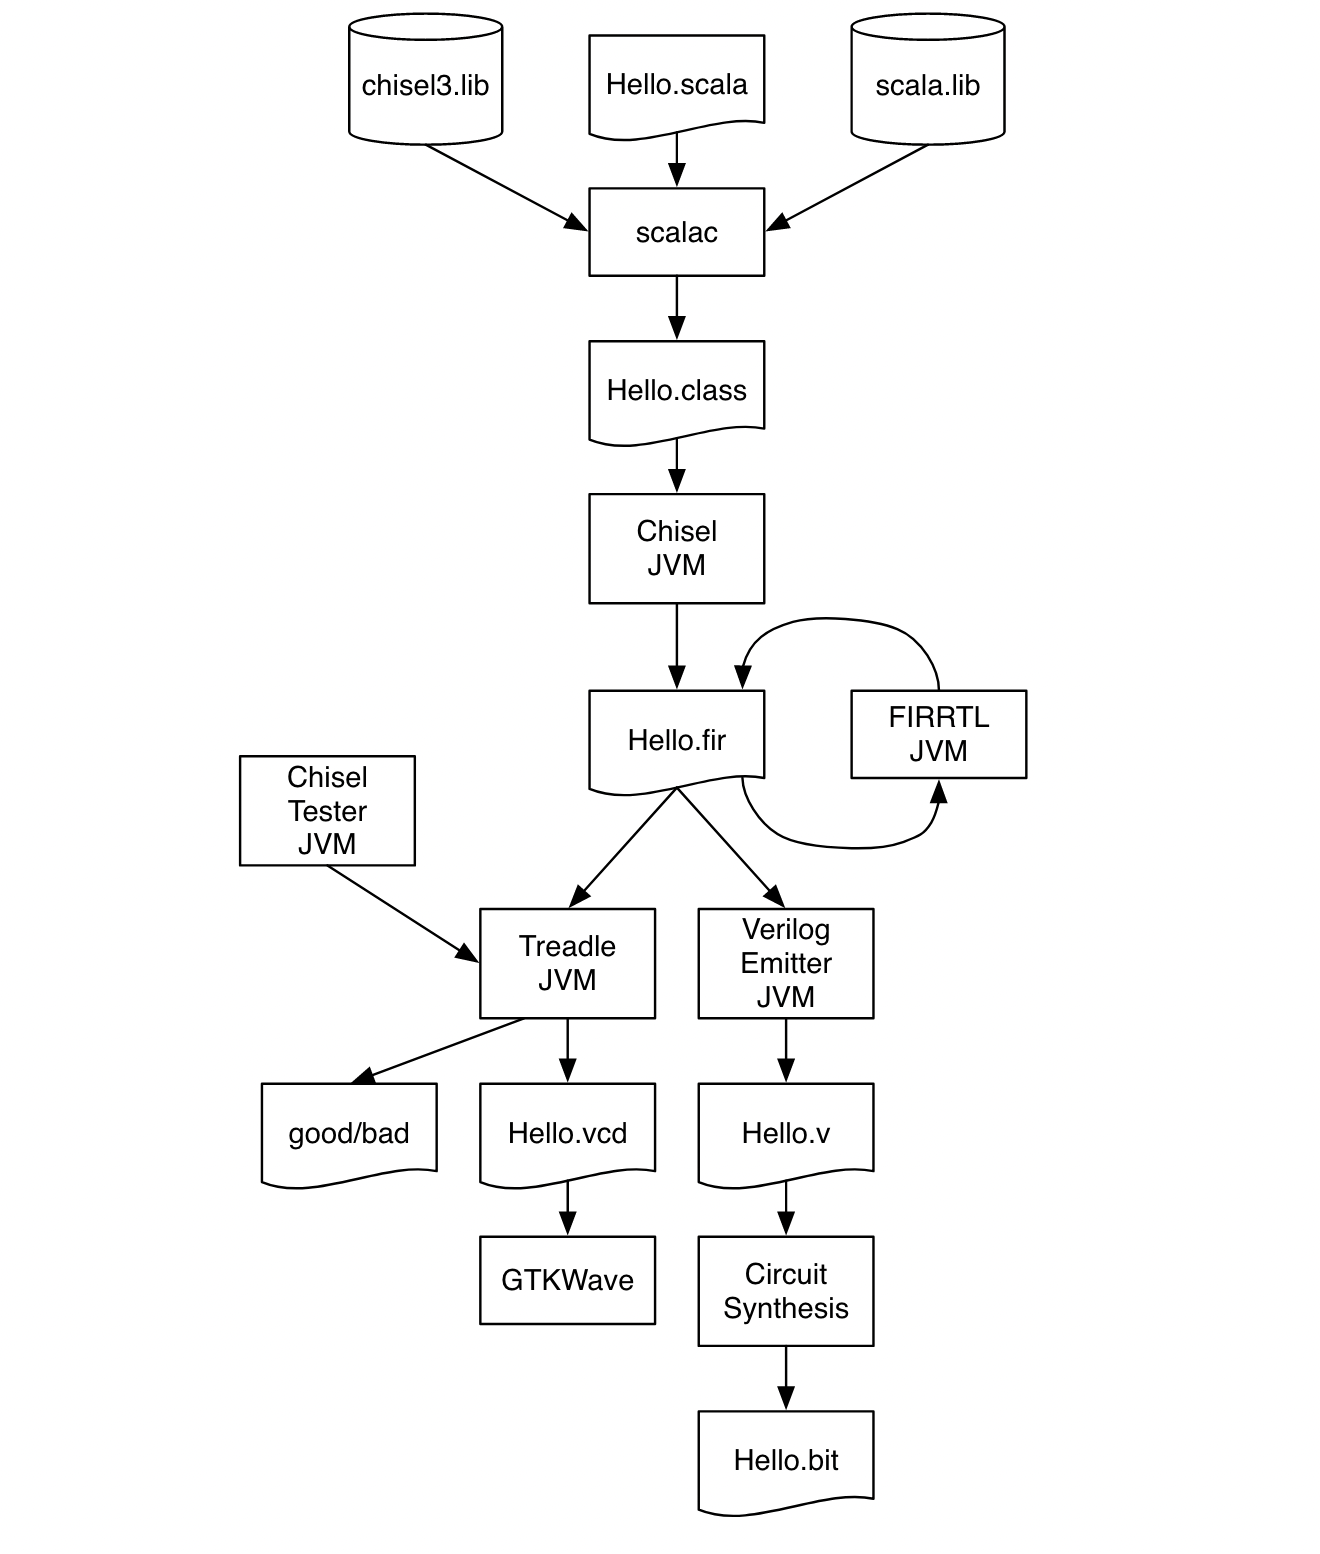
\includegraphics[width=0.5\linewidth]{figures/chisel-tool-flow.png}
    \caption{Chisel 工作流程\cite{chiselbook}}
    \label{fig:chisel}
\end{figure}

\subsection{Rocket Chip}

Rocket Chip 是基于 Chisel 语言的 SoC 生成器,由加州伯克利分校的计算机科学和人工智能实验室开发。Rocket Chip 最大的特点是高度可配置化,支持生成处理器、内存控制器、外设等其他 SoC 组件。Rocket 处理器基于 RISC-V 指令集架构开发,并支持多种指令集扩展,例如基础的整数指令集、乘除扩展、浮点扩展等。

\begin{figure}
    \centering
    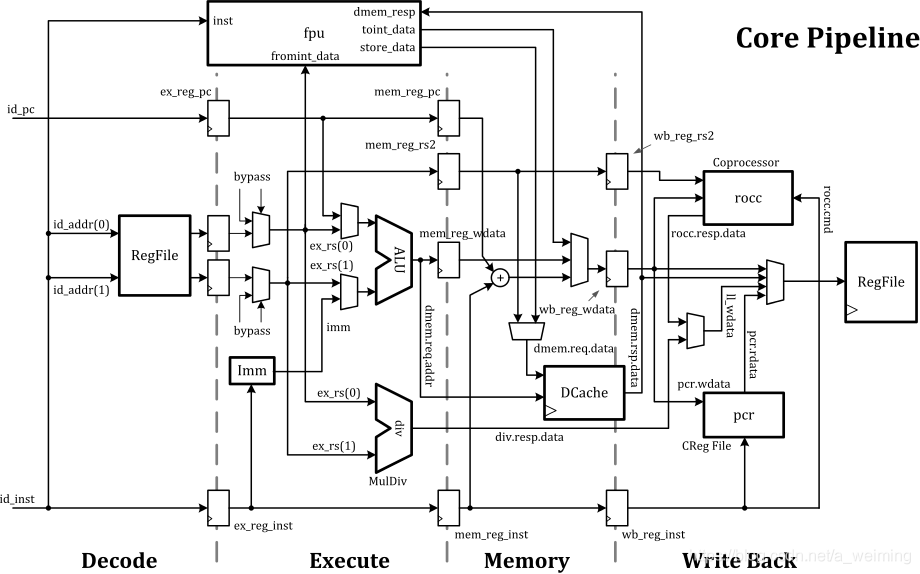
\includegraphics[width=0.8\linewidth]{figures/rocketchip.png}
    \caption{Rocket 处理器数据通路}
    \label{fig:rocketchip}
\end{figure}

\subsection{RoCC}

RoCC (Rocket Custom Coprocessor) \cite{rocc} 是 Rocket Chip 的扩展内容,允许用户添加自定义的协处理器到 Rocket 处理器中来实现加速或其他特殊功能。

RoCC 协处理器通过预定义的接口与 Rocket 处理器进行通信。RoCC 接口定义了一组标准的指令和协议,用于在 Rocket 处理器和 RoCC 协处理器之间传递数据和控制信息,它允许 RoCC 协处理器通过 Rocket 处理器的缓存系统访问内存和外设。

\section{RISC-V N 扩展}

参考设计规范和设计草案,在 rocket/CSR.scala 中添加读写 CSR 的逻辑,需要注意 \Ruip 等多个特权级共用的寄存器需要设置对应特权级的屏蔽位。

参考 M 态中断和异常委托的逻辑,添加 S 态委托到 U 态的逻辑,此外需要在 S 态将已委托给 U 态的中断屏蔽。

在 rocket/IDecode.scala 中添加 \Iuret 的指令解码并将指令解码注册到 decode\_table 中。\Iuret 的功能逻辑比较简单,只需要设置 \Rustatus 中的使能位并重新设置 pc 即可。

\begin{lstlisting}[style=CStyle,language=scala]
    // 读取 uip 寄存器
    val read_uip = read_mip & read_sideleg
    // 委托给 U 态的中断
    val delegateU = Bool(usingUser) && reg_mstatus.prv === PRV.U && delegate && read_sideleg(cause_lsbs) && cause(xLen - 1)
    // U 态的中断
    val u_interrupts = Mux(nmie && reg_mstatus.prv === PRV.U && reg_mstatus.uie, pending_interrupts & read_sideleg, UInt(0))
    // uret 的逻辑
    when (Bool(usingUser) && !io.rw.addr(9) && !io.rw.addr(8)) {
      reg_mstatus.uie := reg_mstatus.upie
      reg_mstatus.upie := true
      ret_prv := PRV.U
      io.evec := readEPC(reg_uepc)
    }
\end{lstlisting}

\section{UINTC 用户态中断控制器}

参考 CLINT 和 PLIC 实现 UINTC 外设,首先定义 device 并指定名称和 compatible ,和 QEMU 中生成设备树的逻辑类似,在这里需要指定 UINTC 连接到 intc ,且需要指定为 interrupt-controller 让 linux 完成初始化。

\begin{lstlisting}[style=CStyle,language=scala]
    val device = new SimpleDevice("uintc", Seq("riscv,uintc0")) {
        override val alwaysExtended: Boolean = true
        override def describe(resources: ResourceBindings): Description = {
            val Description(name, mapping) = super.describe(resources)
            val extra = Map("interrupt-controller" -> Nil,
                "#interrupt-cells" -> Seq(ResourceInt(1)))
            Description(name, mapping ++ extra)
        }
    }
\end{lstlisting}

定义 node 并配置 UINTC 寄存器的读写端口,定义一系列的 RegField 实现读写操作,调用 \mintinline{scala}{node.regmap(opRegFields)} 进行注册:

\begin{lstlisting}[style=CStyle,language=scala]
    val node: TLRegisterNode = TLRegisterNode(
        address = Seq(params.address),
        device = device,
        beatBytes = beatBytes,
        concurrency = 1)

    // 注册 SEND 操作的写端口
    val opRegFields = uirs.zipWithIndex.flatMap { case (x, i) =>
      Seq(sendOffset(i) -> Seq(RegField(64, (),
        RegWriteFn { (valid, data) =>
            x.pending := x.pending | (valid << data(5, 0)).asUInt
            Bool(true)
        })))}
\end{lstlisting}

定义 intnode 连接到 CPU ,在上述 SEND 操作里将 ipi 寄存器对应位置位:

\begin{lstlisting}[style=CStyle,language=scala]
    val intnode: IntNexusNode = IntNexusNode(
        sourceFn = { _ => IntSourcePortParameters(Seq(IntSourceParameters(1,
            Seq(Resource(device, "int"))))) },
        sinkFn = { _ => IntSinkPortParameters(Seq(IntSinkParameters())) },
        outputRequiresInput = false)
    // 拉高 ipi 寄存器
    val ipi = Seq.fill(nHarts) { RegInit(0.U) }
    ipi.zipWithIndex.foreach { case (hart, i) =>
        hart := uirs.map(x => x.pending =/= 0.U && x.active && hartId(x.hartid) === i.asUInt).reduce(_ || _)
    }
    val (intnode_out, _) = intnode.out.unzip
    intnode_out.zipWithIndex.foreach { case (int, i) =>
        int(0) := ShiftRegister(ipi(i)(0), params.intStages) // usip
    }
\end{lstlisting}

关键的是将中断信号连接到对应核的 \FcsrUipUsip ,参考其他信号的处理方法,连接 core.interrupts 和 intSinkNode:

\begin{lstlisting}[style=CStyle,language=scala]
    // freechips.rocketchip.tile.SinksExternalInterrupts
    def csrIntMap: List[Int] = {
        // ...
        val usip = if (usingUser) Seq(0) else Nil
        List(65535, 3, 7, 11) ++ seip ++ usip ++ List.tabulate(nlips)(_ + 16)
    }
    // freechips.rocketchip.subsystem.CanAttachTile
    // 将 intSinkNode 的输入连接到 Rocket 处理器
    def decodeCoreInterrupts(core: TileInterrupts): Unit = {
        // ...
        val usip = if (core.usip.isDefined) Seq(core.usip.get) else Nil
        // ...
        val (interrupts, _) = intSinkNode.in(0)
        (async_ips ++ periph_ips ++ seip ++ usip ++ core_ips).zip(interrupts).foreach { case(c, i) => c := i }
    }
\end{lstlisting}

\section{UIPI 协处理器}

根据 Rocket 处理器的数据通路 \ref{fig:rocketchip} ,RoCC 位于流水线的写回阶段,读写 CSR 时需要考虑写后读冲突,RoCC 读 \Rsuirs 和 \Rsuist 寄存器时需要增加前传逻辑。

\begin{lstlisting}[style=CStyle,language=scala]
    // 前传逻辑,以 suirs 寄存器为例
    when (decoded_addr(CSRs.suirs)) {
        val new_suirs = new SUIRS().fromBits(wdata)
        reg_suirs := new_suirs
        io.uintr.suirs := new_suirs
    }.otherwise {
        io.uintr.suirs := reg_suirs
    }
\end{lstlisting}

在配置中添加 UIPI 协处理器:

\begin{lstlisting}[style=CStyle,language=scala]
    class WithUIPI extends Config((_, _, _) => {
        case BuildRoCC => Seq((p: Parameters) => {
            val module = LazyModule(new UIPI(OpcodeSet.custom3)(p))
            module
        })
    })
\end{lstlisting}

UIPI 协处理器接收译码结果并根据操作码来执行不同处理流程:

\begin{figure}
    \centering
    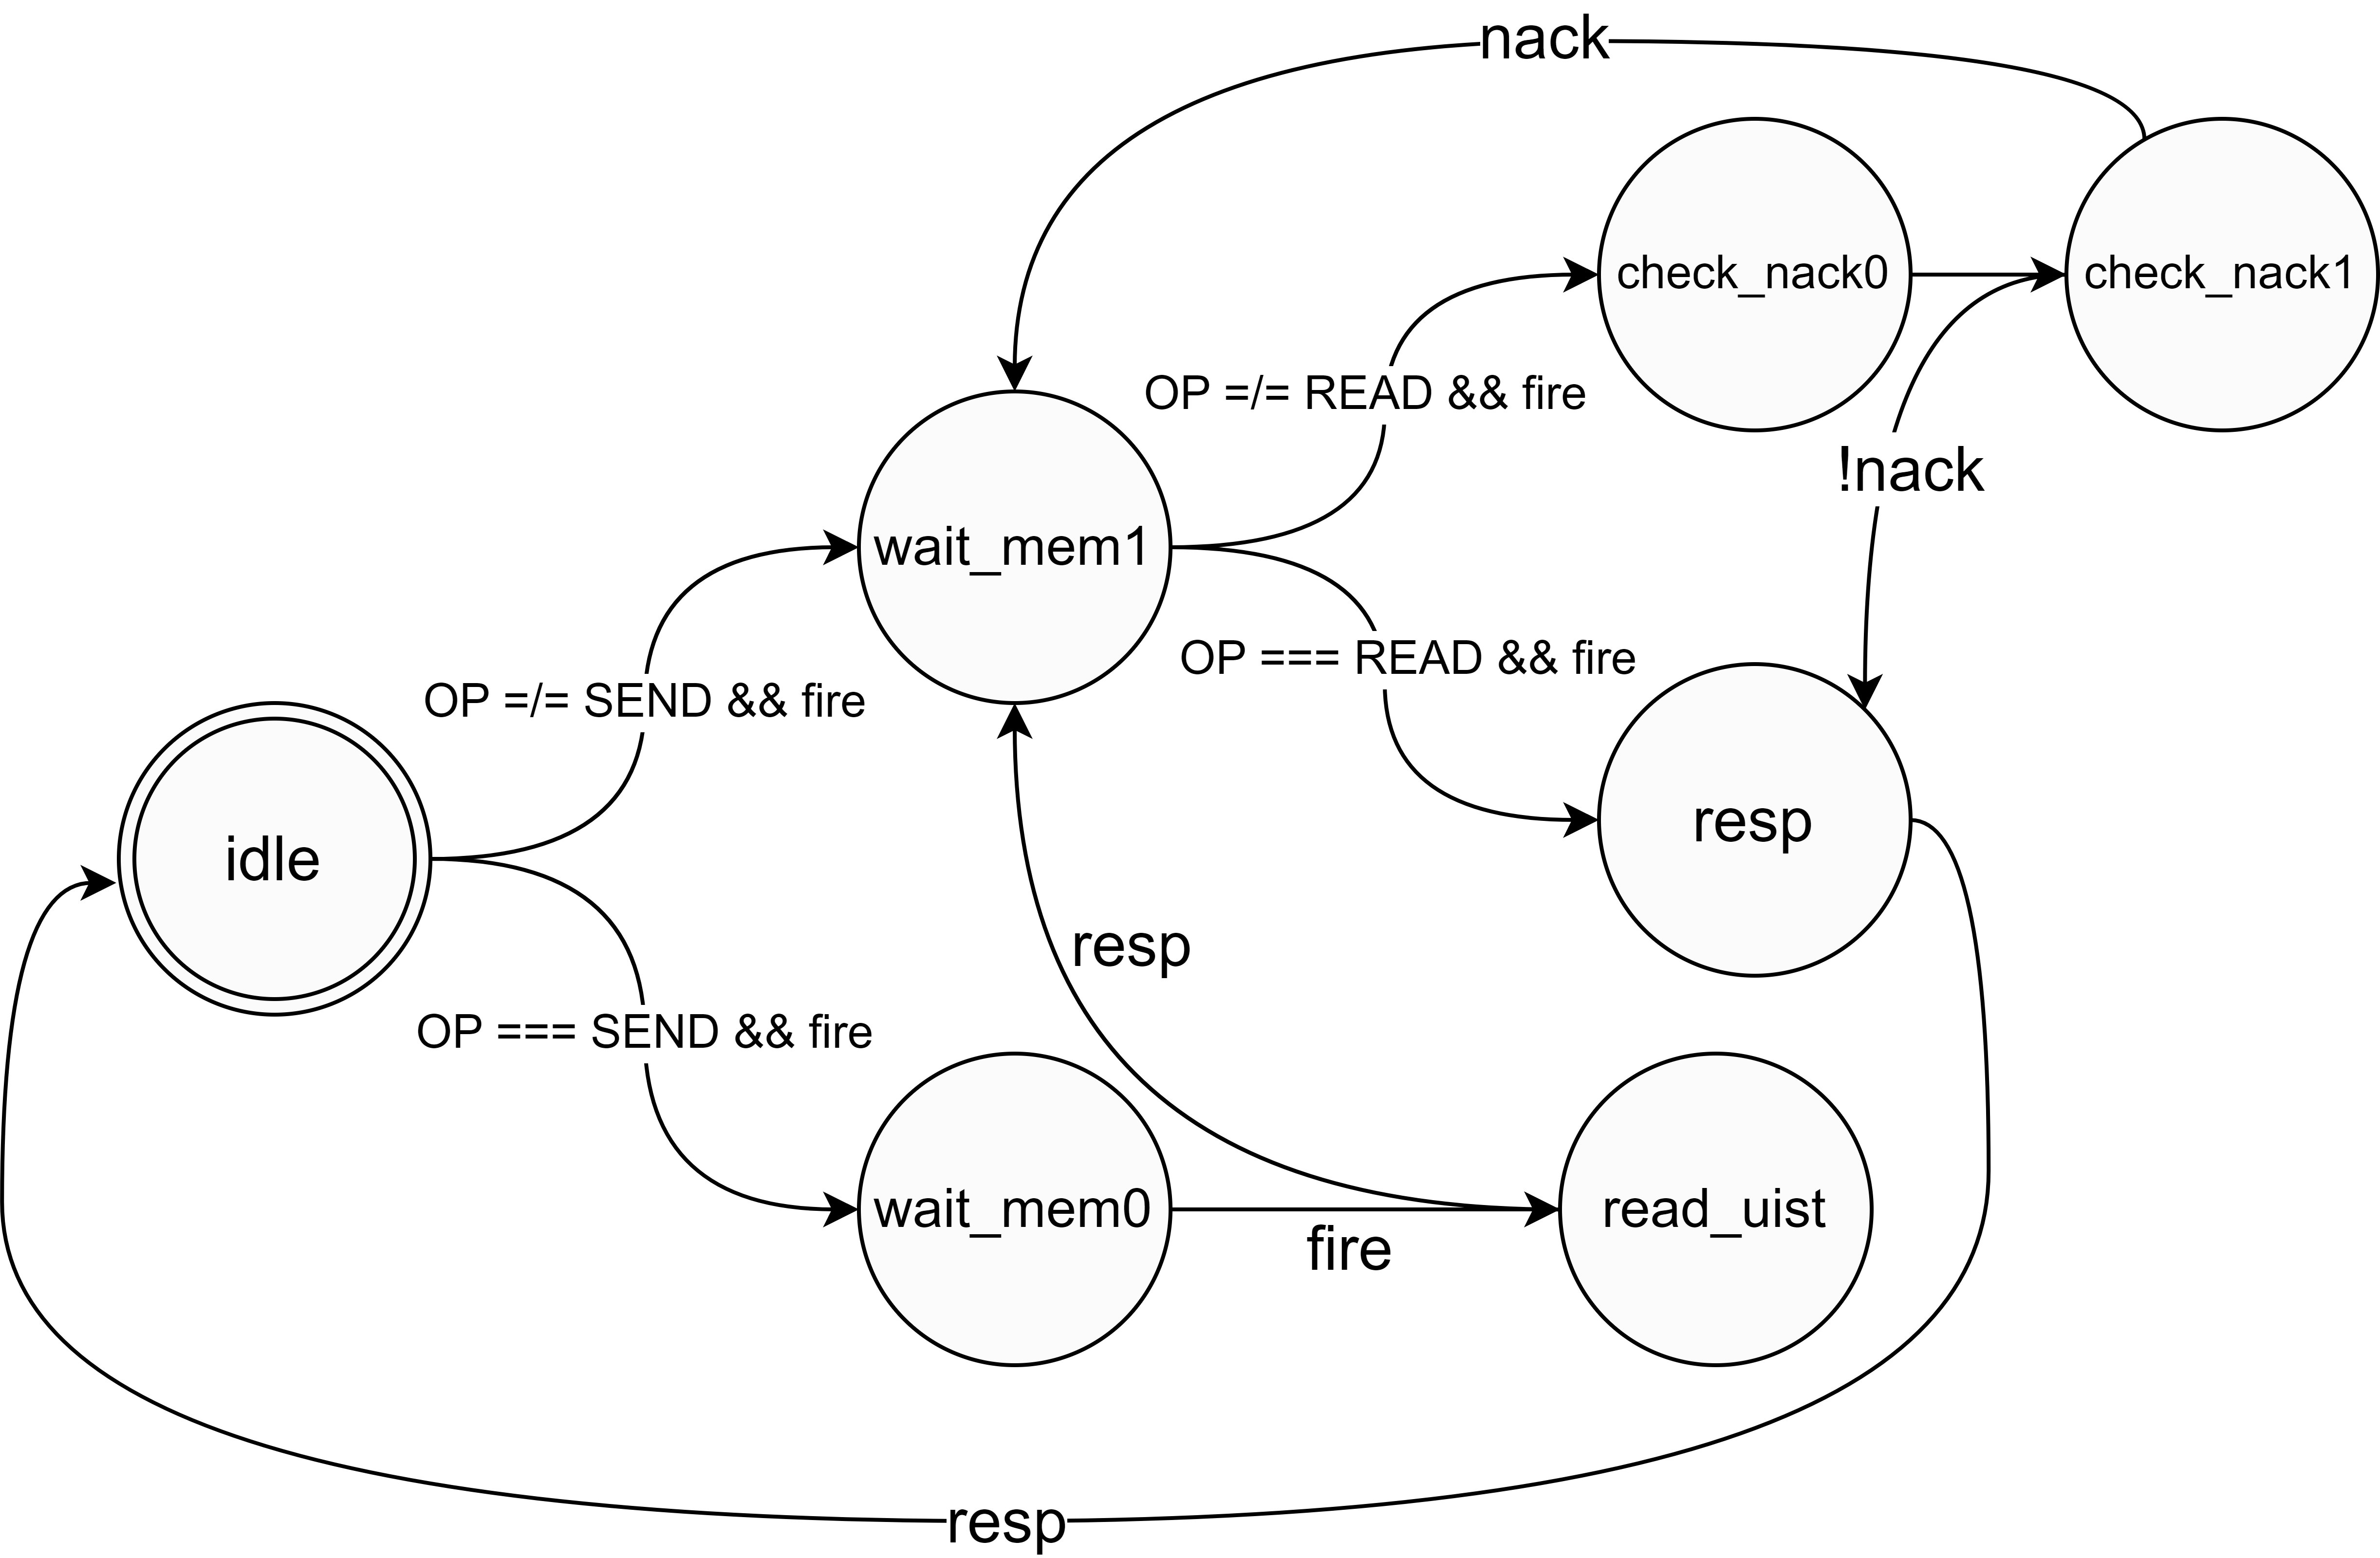
\includegraphics[width=0.5\linewidth]{figures/uintr3.png}
    \caption{UIPI 协处理器工作流程}
    \label{fig:uintr3}
\end{figure}

根据设计草案中对 \Iuipi 指令的描述,UIPI 协处理器要发起至多两次访存请求,其中第二次一定为不经过缓存系统的读或写 UINTC 请求,由于缓存系统考虑了访问外设的请求,在实现逻辑中两次请求会依次经 RoCC 的访存端口发出。此外,对于写外设请求,数据缓存不会拉高 resp 信号,需要在 UIPI 中记录 cycle 并根据数据缓存的响应信号判断最近一次写请求是否成功,若失败则重新发送之前的请求。

SimpleHellaCacheIFReplayQueue 是一个缓存队列模块,用于处理来自 Rocket 处理器和 DMA 设备的读写请求,在默认的实现中被用来缓存多个 RoCC 的读写请求,支持失败读写请求的重试。然而对于写外设请求,队列会持续等待 resp 信号并阻塞。因为目前只有一个 UIPI 协处理器,所以在实际的实现中移除了这个队列。

\section{仿真测试}

基于 riscv-tests 项目\cite{riscvtests}编写了关于 RISC-V 用户态中断扩展的测试程序,用来测试 UINTC 外设和 UIPI 协处理器能否正常工作。

Rocket Chip 提供了多种仿真工具和模拟器,我们采用 verilator 对 RTL 和测试程序进行仿真,可以在仿真结果中查看指令流,还可以查看波形来精确地了解每一个信号的状态。